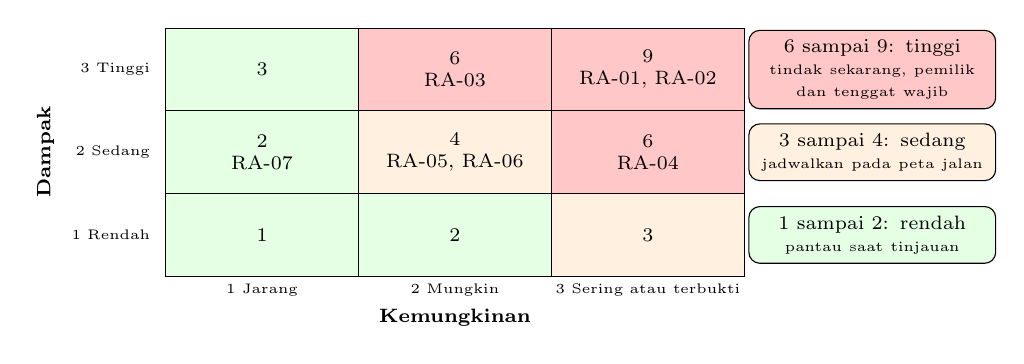
\begin{tikzpicture}[
  font=\scriptsize,
  execute at begin node={\hyphenpenalty=10000\exhyphenpenalty=10000},
  sel/.style={draw, minimum width=2.45cm, minimum height=1.05cm, align=center},
  tinggi/.style={sel, fill=red!22},
  sedang/.style={sel, fill=orange!12},
  rendah/.style={sel, fill=green!10},
  sumbu/.style={font=\scriptsize\bfseries, align=center},
  ket/.style={font=\tiny, align=center}
]
  % Sumbu mendatar kemungkinan, sumbu tegak dampak; skor adalah hasil kali keduanya.
  \node[rendah] at (0,2.1) {3};
  \node[tinggi] at (2.45,2.1) {6\\RA-03};
  \node[tinggi] at (4.9,2.1) {9\\RA-01, RA-02};
  \node[rendah] at (0,1.05) {2\\RA-07};
  \node[sedang] at (2.45,1.05) {4\\RA-05, RA-06};
  \node[tinggi] at (4.9,1.05) {6\\RA-04};
  \node[rendah] at (0,0) {1};
  \node[rendah] at (2.45,0) {2};
  \node[sedang] at (4.9,0) {3};

  \node[ket, anchor=east] at (-1.3,2.1) {3 Tinggi};
  \node[ket, anchor=east] at (-1.3,1.05) {2 Sedang};
  \node[ket, anchor=east] at (-1.3,0) {1 Rendah};
  \node[ket] at (0,-0.7) {1 Jarang};
  \node[ket] at (2.45,-0.7) {2 Mungkin};
  \node[ket] at (4.9,-0.7) {3 Sering atau terbukti};
  \node[sumbu] at (2.45,-1.05) {Kemungkinan};
  \node[sumbu, rotate=90] at (-2.75,1.05) {Dampak};

  \node[draw, rounded corners, fill=red!22, text width=2.9cm, align=center] at (7.75,2.1) {6 sampai 9: tinggi\\{\tiny\mdseries tindak sekarang, pemilik dan tenggat wajib}};
  \node[draw, rounded corners, fill=orange!12, text width=2.9cm, align=center] at (7.75,1.05) {3 sampai 4: sedang\\{\tiny\mdseries jadwalkan pada peta jalan}};
  \node[draw, rounded corners, fill=green!10, text width=2.9cm, align=center] at (7.75,0) {1 sampai 2: rendah\\{\tiny\mdseries pantau saat tinjauan}};
\end{tikzpicture}
